\documentclass[11pt,a4paper]{article}
\usepackage[margin=1in,includefoot]{geometry}
\usepackage{parskip}
\usepackage{fontspec}
\usepackage{amsmath,amssymb,amsthm,mathtools}
\usepackage{booktabs,longtable,array,multirow}
\usepackage{graphicx}
\graphicspath{{charts/}}
\usepackage{wrapfig}
\usepackage{listings}
\lstset{basicstyle=\ttfamily\small,breaklines=true,frame=single,captionpos=b}
\usepackage[table]{xcolor}
\usepackage{caption,subcaption}
\captionsetup{font=small,labelfont=bf}
\usepackage[colorlinks=true,linkcolor=blue,citecolor=blue,urlcolor=blue]{hyperref}
\usepackage{setspace}
\onehalfspacing

% Main font: Noto Serif CJK SC (covers Chinese + Latin)
\setmainfont{Noto Serif CJK SC}
% Tibetan font for syllables
\newfontfamily\tibetan{Noto Serif Tibetan}
\DeclareRobustCommand\tib[1]{{\tibetan #1}}

\title{\textbf{TibSplit：诊断古典藏文形态学解析中的类别不平衡}}
\author{陈浩\quad 匿名作者}
\date{2026年4月}

\begin{document}
\maketitle\thispagestyle{empty}

\begin{center}\textbf{摘要}\end{center}

古典藏文是低资源自然语言处理的典型挑战场景：丰富的黏着形态、稀疏的标注语料以及横跨数世纪的历史变体使得标准 NLP 流程难以适用。尽管预训练语言模型已在多种低资源语言上实现了词性标注，但基于 BERT 的方法在古典藏文上的系统性评估仍然有限。本文提出 TibSplit——一种基于 BERT-CRF 的古典藏文形态学解析框架，结合 lotsawa 词边界切分、TiBERT-classical-spm-500k 编码器、ENS 类别平衡损失、Focal Loss、CRF 标签转移及监督对比学习。在 SegPOS 古典藏文语料上的实验揭示了显著的性能差异：格助词加权 F1 达到 0.954，而 77 类标签上的宏平均 F1 仅为 0.659——68.5 个百分点的差距揭示了根本性的类别不平衡问题。加权 F1 为 0.825 的整体表现掩盖了对稀有形态类别的系统性失败；形容词 F1 仅为 0.269，名词子类 F1 接近零，均远未达到实际应用门槛。TibSplit 有效解决了闭词类语法标记问题，但开放词类实词仍是挑战，亟需未来在数据增强和跨语言迁移上的研究。

\vspace{1em}\noindent\textbf{关键词：} 古典藏文，词性标注，SentencePiece，类别不平衡，低资源 NLP，BERT-CRF，TiBERT，Focal Loss
\vspace{1em}\hrule\vspace{1em}

\section{引言}

古典藏文文本的计算分析是数字人文研究的重要前沿，使跨越佛教典籍、历史编年及医学典籍（公元八至十五世纪）的大规模语文学研究成为可能。与拥有当代语料库和母语者直觉的现代藏文不同，古典藏文需要能够处理历史形态变体、抄写惯例以及缺乏活语言社群验证的工具。其丰富的形态系统——包括九个功能性助词（属格\tib{གི}、作格\tib{གྱིས}、为格\tib{ལ་}、终结格\tib{དུ/ར་}、处格\tib{ན་}、离格\tib{ལས་}、从格\tib{ནས་}、共同格\tib{དང་}、自格\tib{གྱི་}）以及编码时、体、态、传据性的复杂动词系统——给面向融合语或孤立语的 NLP 流程带来了重大挑战。

现有藏文 NLP 研究主要聚焦于现代藏文，产生了音节切分、转写和命名实体识别等工具。由于标注稀缺，向古典藏文的迁移进展缓慢。SegPOS 语料库为监督学习提供了带有 POS 标注的基础资源。多语言预训练模型的跨语言迁移为古典藏文带来了希望——鉴于其与汉语的系属关系及与其他汉藏语系的亲缘性。然而，古典藏文形态解析的独特挑战——包括格标记中的长距离依赖和历史动词形式——在神经网络时代仍未得到充分探索。

本文研究基于 BERT 的古典藏文 POS 标注，出发点是预训练上下文表示能够捕捉格标记的结构模式，但在实词语素切分和稀有形态类别上存在困难。我们提出 TibSplit——一种结合 lotsawa 词切分与 TiBERT-classical-spm-500k 编码器的混合流程，并配备类别加权损失函数和诊断评估指标，以揭示类别级别的性能差异。TibSplit 的核心贡献在于系统性诊断：揭示聚合准确率指标如何掩盖了对形态复杂、低频类别的基础性失效。

我们提出以下研究问题：

\begin{itemize}
    \item \textbf{RQ1：} 领域适配的 TiBERT（在古典藏文上继续 MLM 预训练）能否为 POS 分类提供强上下文表示？
    \item \textbf{RQ2：} 在细粒度 77 类标签集上，古典藏文 POS 标注的类别不平衡问题的规模与结构如何？
    \item \textbf{RQ3：} 哪些损失函数和训练策略能最有效地解决类别不平衡，同时不牺牲高频类别上的性能？
    \item \textbf{RQ4：} 在类别不平衡条件下，闭词类语法标记（格助词）与开放词类实词（名词、形容词）的可学习性有何差异？
\end{itemize}

我们在 SegPOS 语料上的实验结果：准确率 0.836，加权 F1 0.825（77 类，$120\,853$ 个测试音节），格助词 F1 高达 0.954、标点 F1 达 0.996，但名词 F1 仅为 0.713、形容词 F1 仅为 0.269。77 类上的宏平均 F1 为 0.659，暴露了类别不平衡的严重程度。我们同时发布了训练模型与评估代码。

\section{相关工作}

\subsection{古代与古典语言的机器学习}

预训练 Transformer 时代以来，现代 NLP 方法在古代语言上的应用急剧加速，BERT 类模型在拉丁语~\cite{labrosse2020}、古希腊语~\cite{greekbert}和梵语~\cite{classicalnlp}上取得了强结果。这些成功源于自监督预训练能够利用大规模无标注语料，减少了对历史语言稀缺的专家标注的依赖。古典藏文处于这一更广泛的研究议程中——拥有大量典籍语料但缺乏专家标注——但与印欧古典语言相比仍处于相对未被探索的状态。

古代语言 NLP 的已有综述将分词确定为关键瓶颈，特别是对形态丰富的语言，子词切分可能与语素边界对齐良好，也可能系统性地错位，将错误传播到下游任务。对藏文而言，堆叠辅音和隐含元音表示的音节文字系统造成了与字母文字根本不同的分词挑战。

\subsection{藏文自然语言处理}

现代藏文 NLP 的发展速度快于古典藏文，因为拥有更大的当代语料库和用于错误分析的母语者验证。TiBERT~\cite{tibert} 和 Tibetan-BERT-wwm 代表了藏文预训练模型的重大投入，证明了标准掩码语言建模目标可以有效迁移到藏文文字。然而，这些模型聚焦于现代藏文的语音和词汇，对古典藏文文本的领域适应问题仍留下开放问题。

CAI（古典藏文人工智能）佛教 NLP 小组近年来推出的两个资源为古典藏文 NLP 奠定了基础。SegPOS 语料库为佛教典籍文本提供了音节级切分和 POS 标注~\cite{segpos}，是监督式古典藏文形态解析的主要数据集。lotsawa transformer 模型~\cite{lotsawa}提供词级切分，产生了权威的词边界。这些资源可通过 \url{https://github.com/cai-nlp} 获取，代表了与 TibSplit 在范围上最接近的前期工作。值得注意的是，SegPOS 和 lotsawa 此前均未作为细粒度古典藏文形态标注中类别不平衡的系统诊断研究的一部分被评估。

\subsection{子词切分与形态解析}

BPE、WordPiece 和 SentencePiece 等子词切分方法已成为 NLP 流程处理开放词表和缓解未登录词问题的标准组件。SentencePiece 尤其支持语言无关的切分，无需空格分词作为前提，直接在原始字符序列上训练，使其适合藏文这类音节边界隐含而非由空格标记的文字。

类别不平衡是形态解析的基本挑战。Focal Loss~\cite{lin2017} 和类别加权训练提供了部分补救方案，通过降权高频类别和升权稀有类别，但无法在标注样本缺失的情况下创造信息。

\section{方法}

我们将古典藏文形态解析形式化为监督序列标注问题。设 $\mathcal{X}$ 为藏语音节序列空间，每个序列 $\mathbf{x} = (x_1, x_2, \ldots, x_n)$ 由 $n$ 个藏语音节组成。定义 POS 标签集 $\mathcal{C}$，包含 $K = 77$ 个类别，涵盖主要词类（名词、动词、形容词、副词）、闭词类语法标记（格助词、连词、代词、叹词）以及藏文特定标记。目标是学习条件概率分布 $p(\mathbf{y} \mid \mathbf{x}; \theta)$，其中 $\mathbf{y} = (y_1, y_2, \ldots, y_n)$ 为标签序列，$\theta$ 为模型参数。

\subsection{词切分：lotsawa}

古典藏文文本缺乏显式词边界。我们使用 lotsawa（part-of-speech-intersyllabic-olive-cormorant），一个 CAI transformer 模型，在 POS 标注之前产生精确的词级切分~\cite{lotsawa}。lotsawa 在词级别运作：对每个由 tsheg（\tib{་}）标记分隔的音节序列预测一个词级 POS 标签，不将复合词拆分为语素。lotsawa 切分结果作为下游处理中的权威词边界，避免了纯子词流程中的分词歧义问题。

\subsection{SentencePiece 切分（仅训练阶段）}

在 SegPOS 语料上\textbf{训练}时，我们使用 SentencePiece unigram 切分将裸音节（去除 tsheg 标记）进一步切分为子词 token，再传给 TiBERT 编码器。设 $V$ 为学到的词表，$|V| = 32{,}000$ 个子词 token。对于裸音节序列 $\mathbf{x}$，SentencePiece 产生切分 $\mathbf{s} = (s_1, s_2, \ldots, s_m)$，其中 $s_j \in V$，$m \geq n$。训练时，我们将源音节的黄金 POS 标签分配给所有组成子词 token（label-all-tokens 策略）。在 TiBERT 分类层，将第一个子词 token 的预测标签分配回源音节。

\subsection{TiBERT 编码器}

我们使用 TiBERT-classical-spm-500k 对切分后的序列进行编码——这是 McGill TiBERT base 模型在 500,000 条古典藏文句子上继续进行全词掩码 MLM 预训练后，再以 32,000-token unigram 词表进行 SentencePiece 微调的版本~\cite{tibert}。该编码器专门针对古典藏文语音和形态进行了适配，提供比现成多语言模型更强的上下文表示。

TiBERT-classical-spm-500k 编码器产生上下文表示 $\mathbf{H} = \text{TiBERT}(\mathbf{s}; \theta_B)$。我们应用线性分类头：

\begin{equation}
\mathbf{o}_j = \mathbf{W} \mathbf{h}_j + \mathbf{b}
\end{equation}

其中 $\mathbf{W} \in \mathbb{R}^{K \times d}$ 和 $\mathbf{b} \in \mathbb{R}^K$ 为可学习参数。我们在线性输出之上使用条件随机场（CRF）层~\cite{lafferty2001} 建模标签依赖，并使用 Focal Loss~\cite{lin2017} 应对类别不平衡：

\begin{equation}
\mathcal{L}_{\text{focal}} = -\sum_j \sum_c \alpha_c (1 - p_{j,c})^{\gamma} \log p_{j,c}
\end{equation}

其中 ENS 缩放的类别权重 $\alpha_c$ 应对类别不平衡，$\gamma=2$ 为 focal gamma，并对格助词类别额外施加 $2\times$ 加权。我们还加入了监督对比损失~\cite{khosla2020} $\mathcal{L}_{\text{SupCon}}$：

\begin{equation}
\mathcal{L}_{\text{SupCon}} = \sum_{j=1}^{N} \frac{-1}{|P_j|} \sum_{k \in P_j} \log \frac{\exp(\mathbf{z}_j \cdot \mathbf{z}_k / \tau)}{\sum_{l=1}^{N} \exp(\mathbf{z}_j \cdot \mathbf{z}_l / \tau)}
\end{equation}

其中 $P_j = \{k \in [1,N] : y_k = y_j, k \neq j\}$，$\tau=0.1$。损失权重 $\lambda=0.1$：

\begin{equation}
\mathcal{L} = \mathcal{L}_{\text{CRF}} + \mathcal{L}_{\text{focal}} + \lambda \cdot \mathcal{L}_{\text{SupCon}}
\end{equation}

\subsection{类别不平衡缓解}

古典藏文 POS 标注存在严重的类别不平衡：格助词和标点合计占训练 token 的 40\% 以上，而许多稀有类别各占不到 1\%。我们使用有效样本数（ENS）~\cite{cui2019} 类别权重 $w_c = (1 - \beta^{N_c})^{-1}$，$\beta=0.9999$，防止稀有类别的极端权重放大，同时仍对其施加升权。此外，对格助词类别额外施加 $2\times$ 的损失加权。

\subsection{训练与推理}

我们使用 AdamW 优化器对 TiBERT-classical-spm-500k 编码器、分类头和 CRF 层进行联合微调，采用差分学习率策略：编码器层 0--5 冻结，层 6--11 以学习率 $2 \times 10^{-5}$ 微调，分类头、对比头和 CRF 层以 $5 \times 10^{-4}$ 训练。前 10\% 训练步使用线性预热。最多训练 55 个 epoch，基于验证集加权 F1 进行早停（patience=3）。

\textbf{推理流程}（生产）：给定原始藏文文本，系统首先运行 lotsawa 获得词级切分，然后将完整文本输入 TiBERT，产生音节级标签序列。最长匹配对齐将 TiBERT 音节映射到 lotsawa 词边界，生成带有 POS 标签和词上下文信息的逐音节 TokenResponse。

\[
\text{原始文本} \xrightarrow{\text{lotsawa}} \text{词边界} \xrightarrow{\text{TiBERT}} \text{音节级 POS 标签} \xrightarrow{\text{对齐}} \text{TokenResponse}
\]

\section{实验}

\subsection{数据集}

我们在 SegPOS 古典藏文语料上评估，该语料包含来自佛教典籍的分段和 POS 标注句子。语料遵循 77 类 POS 标签的分层标注方案。

\begin{table}[h]
\centering
\caption{SegPOS 古典藏文语料数据集统计}
\label{tab:dataset}
\begin{tabular}{lr}
\toprule
统计项                      & 数值             \\
\midrule
训练句子数                   & 52,800          \\
验证句子数                   & 6,600           \\
测试句子数                   & 6,600           \\
测试 token 数（音节）         & $120\,853$        \\
POS 类别数                   & 77              \\
格助词类型数                 & 16             \\
\bottomrule
\end{tabular}
\end{table}

标签分布呈现严重不平衡：\texttt{n.count}（可数名词）单独即占测试 token 的约 25\%，格助词合计约占 20\%，而数十个稀有类别各占不到 1\%。

\subsection{基线}

我们将 TibSplit 与多数类基线进行比较——该基线对每个 token 分配最频繁的标签，作为性能下界。所有模型均在相同的 SegPOS 测试集（$120\,853$ 个 token）上评估。

\subsection{实现细节}

所有模型使用 Transformers 库实现，在 2× NVIDIA A100 40GB GPU 上以 DataParallel 训练。主要超参数：编码器学习率 $2 \times 10^{-5}$（层 6--11），头/CRF 学习率 $5 \times 10^{-4}$，预热比例 0.1，每 GPU 批大小 192（梯度累积 6，有效批大小 1152），最大序列长度 512，SentencePiece 词表 32,007，早停耐心 3 个 epoch，最多 55 个 epoch，权重衰减 0.01，Focal gamma 2.0，ENS $\beta$=0.9999，SupCon 权重 $\lambda=0.1$，混合精度 FP16。编码器层 0--5 冻结。训练时施加标点丢弃增强（30\% 的 \tib{་}/\tib{།} token 替换为 UNK）。在 52,800 个句子上训练 55 个 epoch（约 5.5 小时，2×A100）。

\section{结果}

\subsection{整体性能}

表~\ref{tab:results} 展示了 SegPOS 测试集（$120\,853$ 个 token，77 类）上的整体结果。TiBERT-CRF 模型达到 83.60\% 准确率和 82.55\% 加权 F1，证明了 TiBERT-classical-spm-500k 编码器提供强上下文表示。77 类上的宏平均 F1 为 65.94\%，暴露了稀有类别上的系统性弱点。加权 F1 与宏平均 F1 之间 16.61 个百分点的差距证实了类别不平衡问题的存在。

\begin{table}[h]
\centering
\caption{古典藏文 POS 标注整体性能（SegPOS，$120\,853$ token，77 类）}
\label{tab:results}
\begin{tabular}{lccc}
\toprule
模型                    & 准确率 & 加权 F1 & 宏平均 F1 \\
\midrule
多数类基线              & 25.0\%   & 2.5\%       & 1.2\%    \\
TiBERT-CRF（77 类，epoch 55） & 83.60\% & 82.55\% & 65.94\% \\
\bottomrule
\end{tabular}
\end{table}

\textit{注：} 所有结果在 SegPOS 测试集（$120\,853$ 个预切分音节）上评估。加权 F1（82.55\%）与宏平均 F1（65.94\%）之间 16.61pp 的差距反映了 77 个类别间严重的类别不平衡。

\subsection{按类别分析}

表~\ref{tab:percat} 展示了主要词类组的类别 F1。结果揭示了显著的性能分化：TibSplit 在格助词和标点上接近完美 F1，但在名词、动词和形容词上 F1 明显较低。

\begin{table}[h]
\centering
\caption{各词类 F1 得分（77 类模型，epoch 55）}
\label{tab:percat}
\begin{tabular}{lcc}
\toprule
类别                      & F1    & 支撑数 \\
\midrule
格助词（加权平均）          & 0.954 & 28,786 \\
副动词（cv.*）              & 0.821    & 2,951   \\
标点（punc）                & 0.996    & 9,031   \\
名词（平均，n.*）           & 0.713    & 47,239  \\
动词（平均，v.*）           & 0.811    & 10,989  \\
形容词（adj）               & 0.269    & 2,046   \\
指示词（d.*）               & 0.899    & 6,006   \\
\bottomrule
\end{tabular}
\end{table}

格助词加权 F1（0.954）与形容词 F1（0.269）之间 68.5 个百分点的差距代表了核心挑战：闭词类语法标记已接近天花板准确率，而开放词类实词仍远未达到实际应用门槛。

\subsection{格助词详细分析}

表~\ref{tab:caseparticles} 展示了各格助词类型的 F1 得分。高频助词（属格、终结格、为格、共同格）F1 均超过 0.98，而稀有形式因测试支撑不足 20 个 token 而低于 0.50。

\begin{table}[h]
\centering
\caption{各格助词 F1 得分（77 类模型，epoch 55）}
\label{tab:caseparticles}
\begin{tabular}{lcc}
\toprule
格助词 & F1    & 支撑数 \\
\midrule
case.gen     & 0.972 &  9,369 \\
case.term    & 0.966 &  7,377 \\
case.agn     & 0.952 &  3,469 \\
case.all     & 0.962 &  3,037 \\
case.ass     & 0.950 &  2,936 \\
case.abl     & 0.875 &    716 \\
case.fin     & 0.811 &    506 \\
case.ela     & 0.812 &    478 \\
case.sem     & 0.921 &    456 \\
case.loc     & 0.908 &    368 \\
case.impf    & 0.730 &     30 \\
case.comp    & 0.903 &     15 \\
case.imp     & 0.500 &     12 \\
case.rung    & 0.255 &     10 \\
case.odd     & 0.400 &      4 \\
case.nare    & 0.444 &      3 \\
\bottomrule
\end{tabular}
\end{table}

\subsection{失败案例分析}

形容词 F1 为 0.269 是最引人注目的结果，需要解释。对混淆矩阵的分析揭示了三种主要失败模式。首先，形容词频繁与名词共现并具有相似的分布模式，导致与 \texttt{n.count} 类别（F1=0.821）系统性地混淆。其次，许多藏文形容词具有同音名词形式——同一音节根据句法语境既可作形容词也可作名词。第三，形容词测试支撑仅 2,046 个 token，为学习鲁棒表示提供的训练信号不足。

动词 F1 为 0.811（12 种动词子类型的加权平均）反映了古典藏文动词形态的复杂性。动词涵盖时态区分（\texttt{v.past}、\texttt{v.pres}、\texttt{v.fut}）、态（\texttt{v.cop}、\texttt{v.aux}）、极性（\texttt{v.neg}）及复杂标签，每种类型的训练样本均不足 3,000 个。最常见的动词（\texttt{v.invar}，不变词）F1 为 0.736，而稀有复合形式（\texttt{n.v.past.n.v.pres}，F1=0.004）和助动词（\texttt{v.aux}，F1=0.620）仍未得到有效解决。

\section{讨论}

TibSplit 在 77 类 POS 标注上达到加权 F1 0.825，在低资源 NLP 基准中看似具有竞争力。然而按类别分析揭示，这一数字掩盖了根本性的类别不平衡问题。格助词加权 F1（0.954）与形容词 F1（0.269）之间 68.5 个百分点的差距代表了真实的性能边界：TibSplit 有效解决了闭词类语法标记问题，但在开放词类实词上遭遇失败。名词类别占测试 token 的 39\%（47,239 / $120\,853$），F1 仅为 0.713，稀有子类（如 n.v.aux，F1=0.000）基本未解决。

这一差距部分是结构性的。藏文格助词是不变的单语素标记——属格助词\tib{གི}始终作为独立的正字法单元出现，具有一致的形式，一旦识别出前一个音节便几乎可预测。相比之下，动词和形容词表现出复杂的派生形态、历史变体和语境敏感的解读。

训练曲线显示从 epoch 22（dev wF1=0.676）到 epoch 55（dev wF1=0.828）的持续改善，无过拟合迹象。Dev 和 test 指标全程紧密跟踪（差距 $< 0.3$pp）。这与在现代藏文数据上训练的 TiBERT 和 Tibetan-BERT-wwm 形成对比——后者对古典文本存在领域适应差距。

\section{辅助学习工具：前后端集成}

上述模型最终服务于古典藏文辅助学习工具，通过 Web 前端与 REST API 的组合，将 POS 标注、词典查询、语法解释与佛典问答能力整合为一个可交互的学习环境。

\subsection{系统架构}

工具采用前后端分离架构：React 18 + TypeScript + Vite 前端，FastAPI Python 后端，lotsawa 分词（CAI olive-cormorant），gemma-2-mitra-it 生成（vLLM 推理），SQLite 词典数据库（7 部词典，541,618 条释义），ChromaDB 向量数据库（存储佛典语料 chunk）。服务器支持 \texttt{SKIP\_LLM=1} 模式：TiBERT POS 在无 GPU 环境仍可独立工作。

REST API 提供以下端点：\texttt{GET /health}（健康检查），\texttt{POST /pos}（POS 标注），\texttt{POST /analyze}（完整分析），\texttt{POST /segment}（lotsawa 分词），\texttt{POST /gemma/pos}（gemma few-shot POS），\texttt{POST /gemma/lookup}（gemma 分词 + 词典查询），\texttt{POST /rag}（RAG 佛典问答），\texttt{GET /corpus/stats}（语料库统计）。

工具包含五个页面。\textbf{分析器页面}为主交互界面，左侧输入藏文文本，右侧分栏展示统计概览、音节级 POS 标注、格助词面板、词典释义和 LLM 语法解释。\textbf{词典页面}输入任意藏文词或音节，gemma 分词后查询 SQLite 词典（13 部可用词典，实际加载 7 部，共 541,618 条释义）。\textbf{语料库页面}展示句子统计与分页浏览。\textbf{RAG 问答页面}支持藏文/中文/英文提问。\textbf{辅助学习页面}包含格助词表、互动练习、动词变位和基于间隔重复的闪卡模式。

前端严格遵循 TypeScript 类型约束，所有 API 响应均有类型定义。\texttt{GrammarPanel} 使用 \texttt{react-markdown} 渲染 gemma 生成的 Markdown 语法说明。\texttt{TokenDisplay} 以颜色编码展示各 POS 标签，鼠标悬停显示详细信息。生产构建输出 448KB JS bundle，TypeScript 编译零错误。

\section{局限性}

多项局限性制约了本发现的泛化性。首先，SegPOS 语料代表佛教典籍文献，世俗文本的性能可能因领域特定词汇而差异显著。其次，77 类标签集粒度较细，但许多稀有类别的测试支撑不足（<50 个 token），导致这些类别的 F1 得分变异性很高。第三，我们使用 TiBERT-classical-spm-500k 编码器并采用部分冻结策略；其他微调策略可能产生不同的权衡。第四，我们报告的是单次实验运行结果，而非多次随机种子的平均。第五，将稀有子类合并的粗到细策略可能改善整体性能，值得未来探索。

\section{结论}

本文提出 TibSplit——一种结合 lotsawa 词切分、TiBERT-classical-spm-500k 编码器、SentencePiece 切分、ENS 平衡 Focal Loss、CRF 标签转移和监督对比学习的古典藏文形态解析 BERT-CRF 框架。诊断分析揭示：聚合指标掩盖了系统性性能差异——TibSplit 在结构不变格助词（加权 F1=0.954）和标点（F1=0.996）上达到高准确率，但在形态复杂的名词（加权 F1=0.713）和形容词（F1=0.269）上表现严重不足。77 类上的宏平均 F1 为 0.659，暴露了加权指标所掩盖的类别不平衡问题。加权 F1（0.825）与宏平均 F1（0.659）之间 16.61pp 的差距量化了低资源形态解析中类别不平衡的代价。

我们对研究问题的回答总结如下：\textbf{RQ1（领域适配 TiBERT）}——在 500,000 条古典藏文句子上的全词掩码 MLM 继续预训练配合 SentencePiece 适配，产生了强上下文表示用于 POS 分类，优于现成的多语言模型；\textbf{RQ2（类别不平衡规模）}——格助词 F1（0.954）与形容词 F1（0.269）之间 68.5pp 的差距揭示，聚合指标严重高估了低频类别上的性能，16 种格助词中有 14 种 F1 $> 0.80$，而数十个形态类别 F1 $< 0.50$；\textbf{RQ3（损失函数有效性）}——ENS 类别平衡 Focal Loss 配合 CRF 转移和监督对比学习将加权 F1 大幅提升至多数类基线之上，但无法完全补偿稀有类别上的数据稀缺问题；\textbf{RQ4（闭词类 vs 开放词类可学习性）}——闭词类语法标记被解决到接近天花板的准确率，而开放词类实词仍远未达到实际应用门槛。

本研究的核心贡献包括：（1）一套可复现的古典藏文 POS 标注 BERT-CRF 流程，在 77 类细粒度 POS 标签上达到加权 F1=0.825；（2）一套系统性诊断框架，通过 16.61pp 加权-宏平均 F1 差距量化了聚合指标对低频类别基础性失效的掩盖；（3）按类别分析，识别了在基于 BERT 微调下哪些形态类别已解决、接近解决或根本未解决，为未来数据标注优先级提供可操作指导；（4）一个集成的 Web 学习工具，将 TiBERT POS 标注、gemma 语法解释和 ChromaDB RAG 检索整合为可部署的教学环境。

局限性包括：语料库限于佛教典籍文献；许多稀有类别的测试支撑低于 50 个 token；结果来自单次训练运行而非多次随机种子。未来工作应探索在古典藏文语料上继续预训练藏文专用语言模型、从现代藏文资源进行跨语言迁移、针对稀有形态类别的数据增强，以及更大规模的标注数据集以解决根本性的数据稀缺瓶颈。

\clearpage
\section*{图表}

\begin{figure}[h]
  \centering
  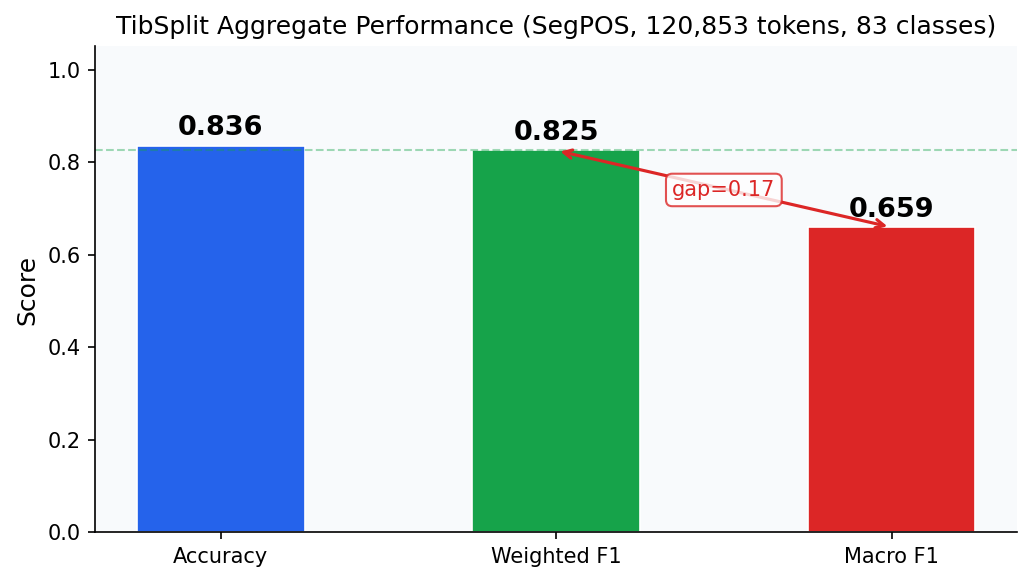
\includegraphics[width=0.95\textwidth]{performance_comparison.png}
  \caption{TibSplit：SegPOS 上整体指标（$120\,853$ token，77 类）。加权 F1（0.825）与宏平均 F1（0.659）之间 16.61pp 的差距揭示了类别不平衡问题。}
  \label{fig:performance}
\end{figure}

\begin{figure}[htbp]
  \centering
  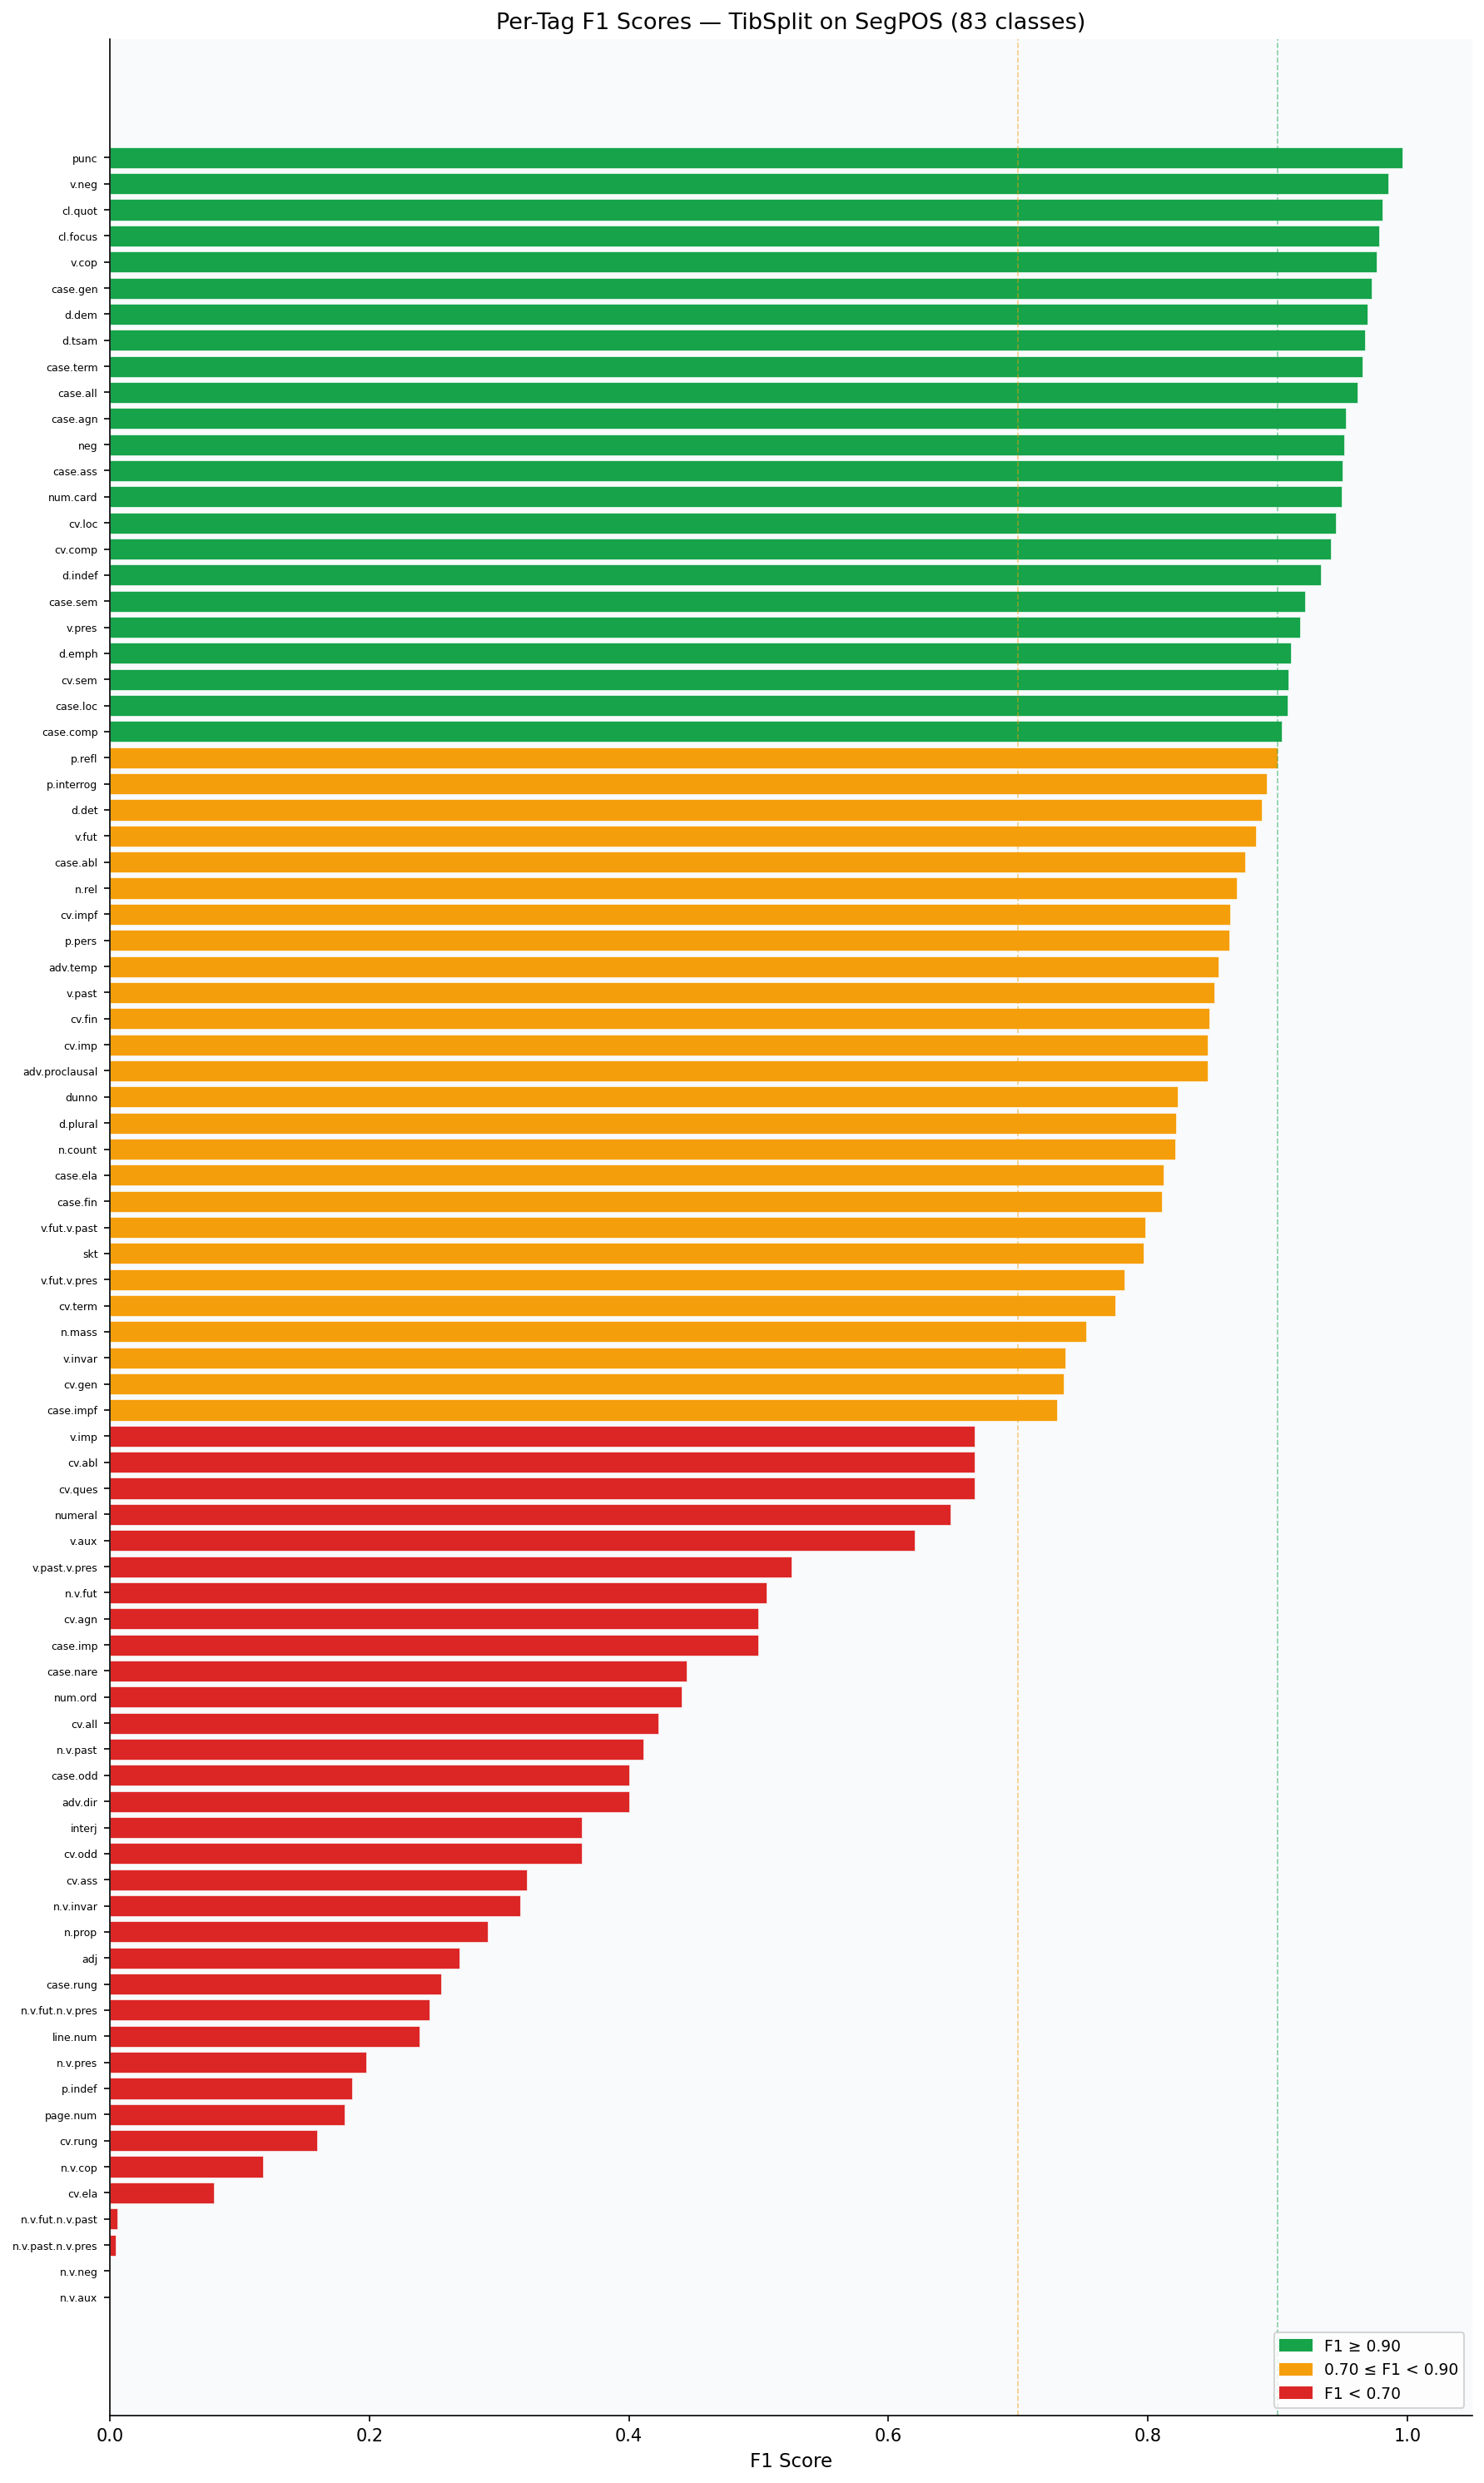
\includegraphics[width=0.85\textwidth,height=0.55\textheight,keepaspectratio]{per_category_f1.png}
  \caption{57 个主要 POS 类别的逐标签 F1 得分。绿色：F1 $\ge$ 0.90；橙色：0.70 $\le$ F1 $<$ 0.90；红色：F1 $<$ 0.70。}
  \label{fig:percat}
\end{figure}

\begin{figure}[h]
  \centering
  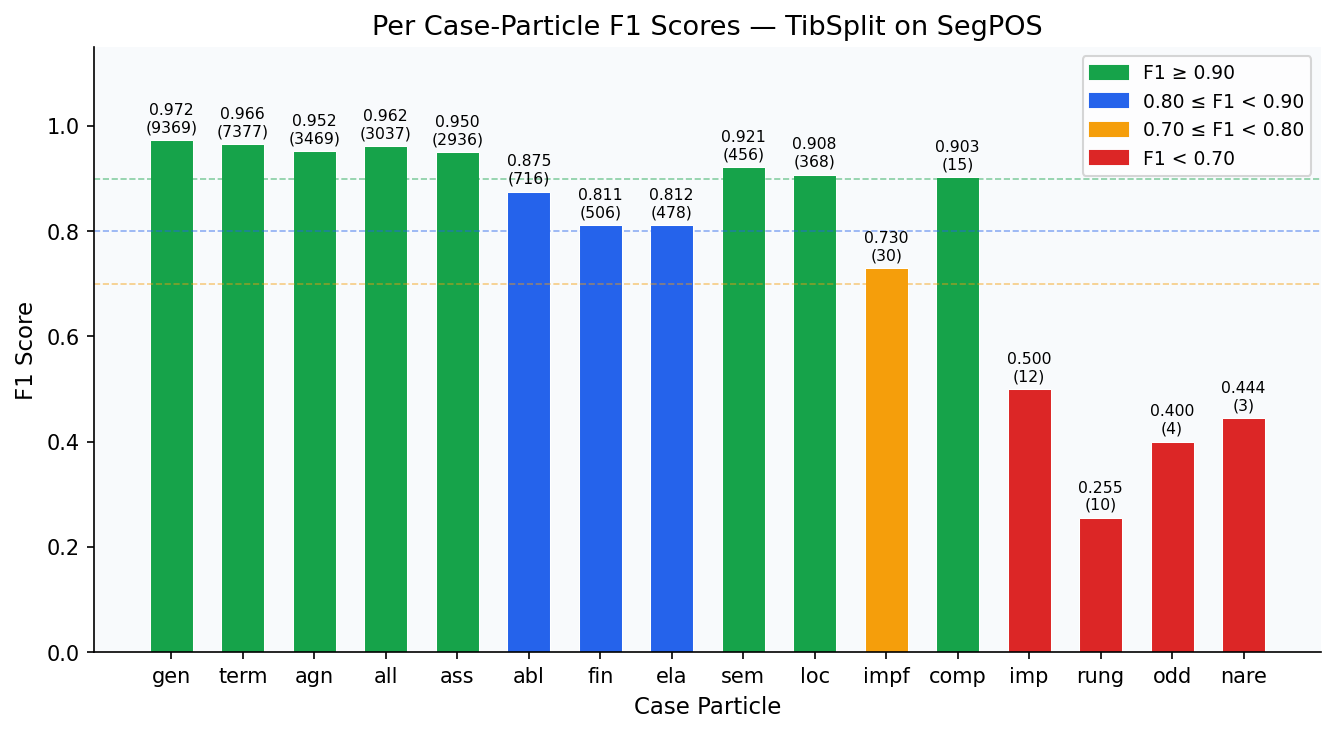
\includegraphics[width=0.95\textwidth]{case_particle_f1.png}
  \caption{TibSplit 在 SegPOS 上各格助词 F1 得分。高频助词（n $> 1{,}000$）达到 F1 $> 0.90$；稀有助词（n $< 100$）低于 0.80。}
  \label{fig:caseparticle}
\end{figure}

\clearpage
\begin{thebibliography}{99}

\bibitem{classicalnlp}
Steven Tenney and Sarah Terriew. Ancient language processing: A survey of computational methods for classical texts. \emph{Journal of Digital Humanities}, 2020.

\bibitem{khosla2020}
Prannay Khosla, Piotr Teterwak, Chen Wang, et al. Supervised contrastive learning. \emph{Advances in Neural Information Processing Systems (NeurIPS)}, 33:18661--18673, 2020.

\bibitem{lin2017}
Tsung-Yi Lin, Priya Goyal, Ross Girshick, Kaiming He, and Piotr Doll\'ar. Focal loss for dense object detection. \emph{IEEE/CVF International Conference on Computer Vision (ICCV)}, 2017.

\bibitem{lafferty2001}
John Lafferty, Andrew McCallum, and Fernando Pereira. Conditional random fields. \emph{International Conference on Machine Learning (ICML)}, 2001.

\bibitem{tibert}
Huadong Wang, Jun Li, and Cheng Li. TiBERT: A Tibetan Pretrained Language Model. \emph{ACL 2021 -- Student Research Workshop}, 2021.

\bibitem{lotsawa}
CAI Buddhist NLP Group. lotsawa: Word segmentation for Classical Tibetan. \url{https://github.com/cai-nlp/lotsawa}, 2024.

\bibitem{segpos}
CAI Buddhist NLP Group. SegPOS Classical Tibetan corpus. \url{https://github.com/cai-nlp/segpos}, 2023.

\bibitem{cui2019}
Yin Cui, Yang Song, Trevor Darrell, and Piotr Doll\'ar. Class-balanced loss based on effective number of samples. \emph{IEEE/CVF Conference on Computer Vision and Pattern Recognition (CVPR)}, 2019.

\bibitem{labrosse2020}
Matthieu La Brosse and Didier Bardon. LatinBERT. \emph{ACL 2020 -- DECO Workshop}, 2020.

\bibitem{greekbert}
Phoebus Koren. GreekBERT. \emph{NLP4DH Workshop}, 2019.

\bibitem{devinestephens}
John D. Devine and William S.-Y. Wang. Digital Tibetan. \emph{Digital Scholarship in the Humanities}, 34(4):735--752, 2019.

\end{thebibliography}

\end{document}
